\chapter{Inleiding}
\label{inleiding}
%%%%%%%%%%%%%%%%%%%%%%%%%%%%%%%%%%%%%%%%%%%%%%%%%%%%%
%          Waarom configuratiemanagement?           %
%%%%%%%%%%%%%%%%%%%%%%%%%%%%%%%%%%%%%%%%%%%%%%%%%%%%%
Configuratiebeheergereedschappen zijn ontwikkeld om het leven van systeembeheerders makkelijker te maken.
De serverinfrastructuren die ze moeten onderhouden worden steeds uitgebreider en complexer.
Manueel elke server configureren kost niet alleen teveel tijd maar is ook erg foutgevoelig.
Het gebruik van scripts is al een stap in de goede richting maar is nog steeds niet voldoende.
Als bijvoorbeeld ssh gebruikt wordt om een reeks servers up te daten en \'e\'en ervan is niet beschikbaar is er plots een verschil tussen systemen die eigenlijk dezelfde configuratie zouden moeten hebben. \todo{Herschrijven}

Een andere manier om een verzameling gelijkaardige machines van hun initi\"ele configuratie te voorzien is het gebruik van images.
Daarbij wordt eerst \'e\'en machine manueel geconfigureerd en daarna de volledige set-up gekloond naar de rest van de servers.
Deze methode werkt niet meer voor het verdere onderhoud van de configuraties.
%http://sysadvent.blogspot.be/2011/12/day-19-why-use-configuration-management.html

%%%%%%%%%%%%%%%%%%%%%%%%%%%%%%%%%%%%%%%%%%%%%%%%%%%%%
%          Overgaan naar de cloud                   %
%%%%%%%%%%%%%%%%%%%%%%%%%%%%%%%%%%%%%%%%%%%%%%%%%%%%%
Dit onderhoudsprobleem komt nog prominenter voor als de infrastructuur niet lokaal maar in de cloud gehost wordt.
Een groot voordeel van werken in de cloud is de flexibiliteit waarmee servers kunnen toegevoegd en weggenomen kunnen worden.
Dit proces gebeurt vaak zelfs automatisch waardoor manuele configuratie helemaal geen optie meer is. \todo{source?}
In een dergelijke omgeving is een tool die uit zichzelf de volledige infrastructuur kan beheren bijna een noodzaak.
Configuratiebeheergereedschappen (of CMS: Configuration Management Software, vanaf nu zal deze term gebruikt worden) zoals
IMP\footnote{http://people.cs.kuleuven.be/~bart.vanbrabant/impdoc/index.html},Puppet\footnote{http://puppetlabs.com/}, CFEngine\footnote{http://cfengine.com/},\ldots laten toe op een effici\"ente manier IT infrastructuren op te zetten en onderhouden.

%%%%%%%%%%%%%%%%%%%%%%%%%%%%%%%%%%%%%%%%%%%%%%%%%%%%%
%          Werking huidige tools                    %
%%%%%%%%%%%%%%%%%%%%%%%%%%%%%%%%%%%%%%%%%%%%%%%%%%%%%
De gebruiker van een dergelijke tool specifi\"eert eerst een model dat de gewenste toestand van de volledige infrastructuur beschrijft.
Dit model bestaat uit een oplijsting van machines met de gewenste aanwezige resources (bestanden, mappen, services,\ldots) die ze moeten aanbieden.
%Dit model is zo bij de huidige tools, niet echt bij IMP
Een eenvoudige voorbeeldconfiguratie is de LAMP-stack: een Linuxinstallatie met daarop een Apache webserver, de MySQL databaseservice en PHP.

Bij het uitrollen van een configuratie (een "deployment run") inspecteert de CMS de huidige toestand van elke machine en vergelijkt ze met de gewenste toestand.
Als er een verschil is maakt de CMS de nodige aanpassingen, indien niet onderneemt ze geen actie.
De beheerder van de verzameling systemen moet dus na het opstellen van de initi\"ele configuratie zelf geen stappen meer ondernemen om te verzekeren dat de gewenste situatie bereikt wordt.
Als er later nog aanpassingen moeten gebeuren moet enkel het model aangepast worden en een nieuwe deployment run gestart worden, manueel inloggen op elke server is niet meer nodig.


%%%%%%%%%%%%%%%%%%%%%%%%%%%%%%%%%%%%%%%%%%%%%%%%%%%%%
%          Dependencies gebruiken gaat beter        %
%%%%%%%%%%%%%%%%%%%%%%%%%%%%%%%%%%%%%%%%%%%%%%%%%%%%%
Een belangrijk aspect van elk gedistribueerd systeem zijn de afhankelijkheden die bestaan tussen de verschillende delen van dat systeem.
In het voorbeeld van de LAMP-stack heeft de webserver naast PHP-mogelijkheden ook een werkende database nodig, anders kan deze niet alle functionaliteit aanbieden.
\begin{figure}
    \label{fig:lamp_dep}
    \begin{center}
    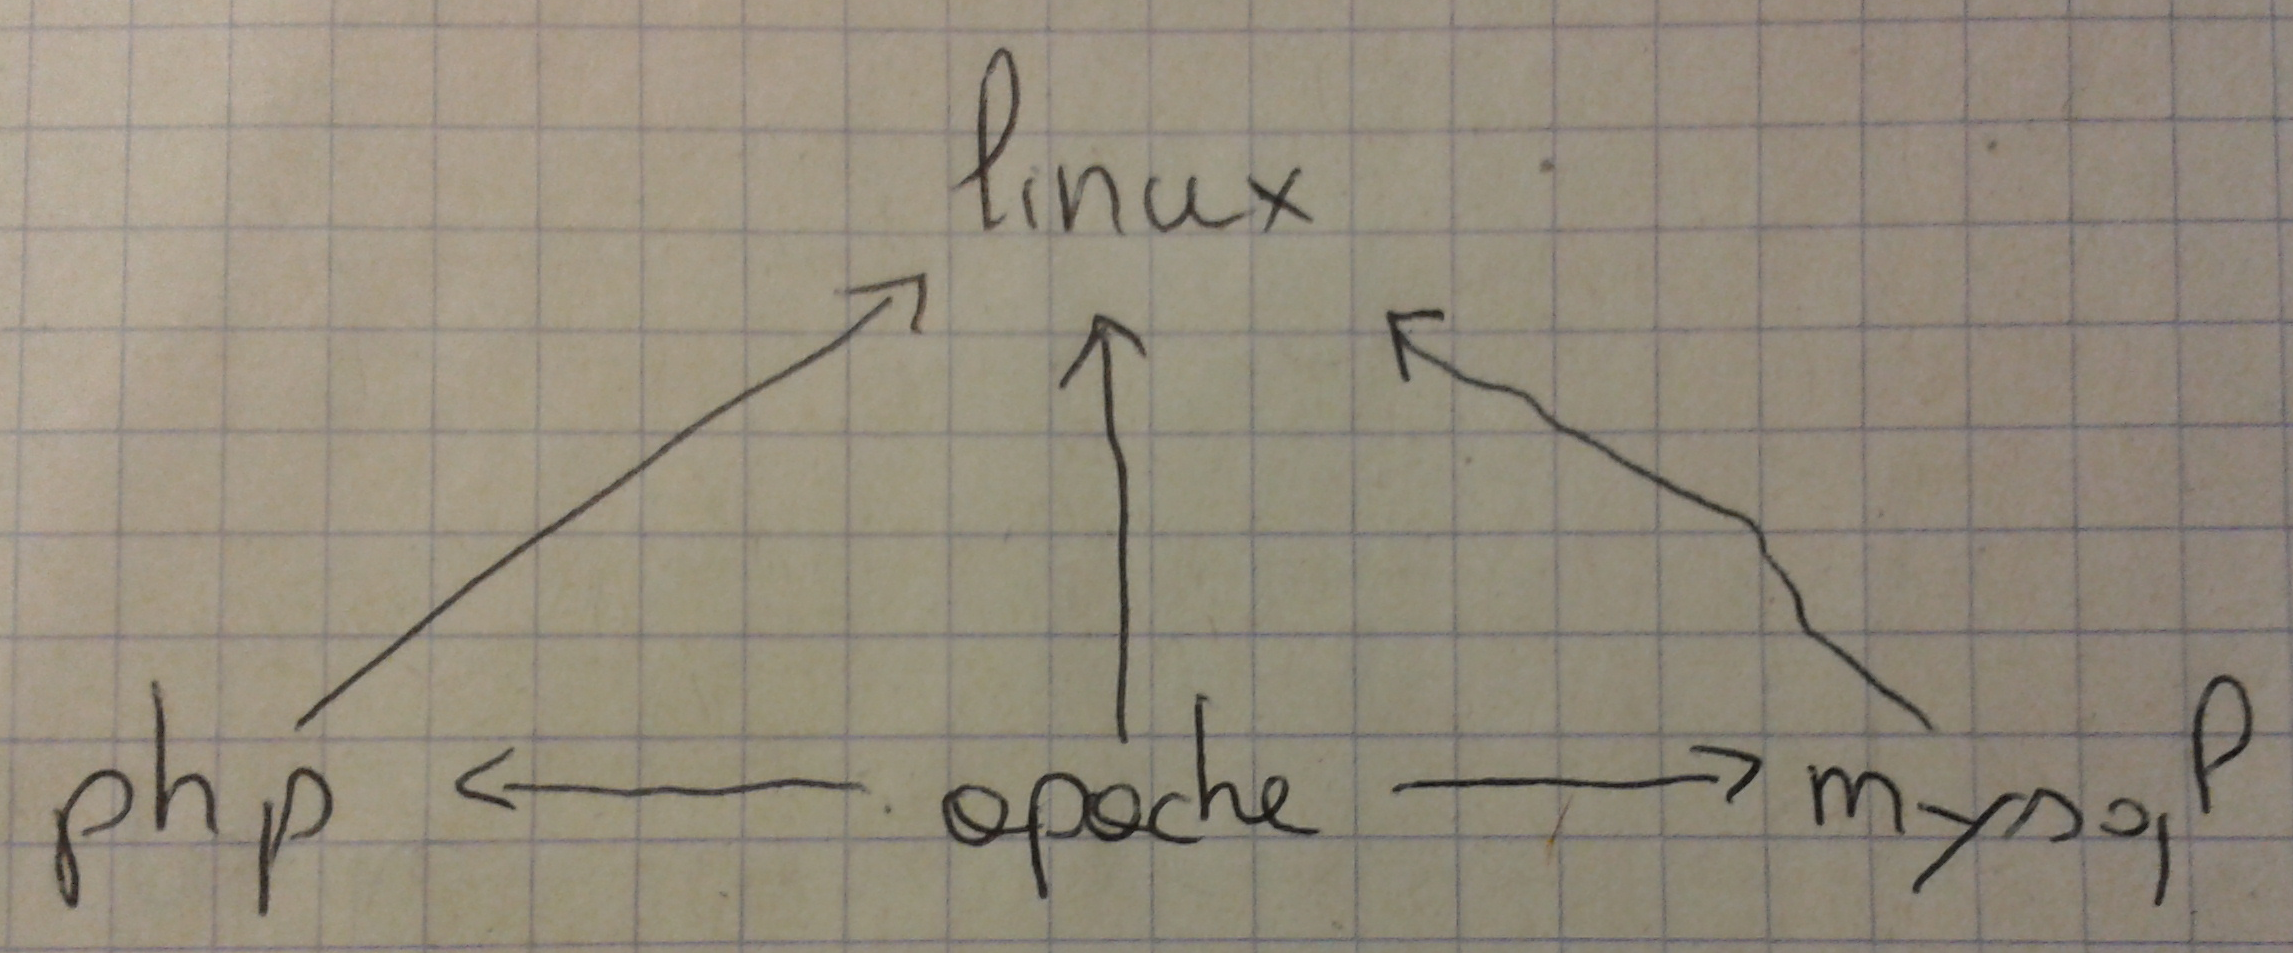
\includegraphics[width=0.6\textwidth]{images/lamp_dep.png}
    \caption{Grafische voorstelling van de afhankelijkheden binnen een LAMP-stack}
    \end{center}
\end{figure}
Als deze afhankelijkheden niet gespecifi\"eerd worden in het model kan de CMS er ook geen rekening mee houden.
De tool kan dus het model in een foute volgorde verwerken: eerst de webserver, dan php en uiteindelijk de database.
De webserver zal bij het opstarten proberen te verbinden met de database, maar deze is nog niet online.
Een op het eerste zicht succesvolle deployment run kan dus leiden tot een configuratie die niet volledig werkt.

In vergelijking met de beginsituatie is de toestand van de setup na \'e\'en run wel al minder afwijkend van de gewenste situatie:
de CMS zal nooit aanpassingen maken die zorgen voor een configuratie die verder afwijkt van het model dan voorheen.
Na een paar iteraties zal uiteindelijk altijd de gewenste configuratie bereikt worden.
Het aantal iteraties is afhankelijk van de hoeveelheid afhankelijkheden die bestaan maar niet aanwezig zijn in het model.
De kans bestaat wel altijd dat met wat geluk de CMS een willekeurige maar effici\"ente volgorde kiest.
\begin{figure}
    \label{fig:convergentie}
    \begin{center}
    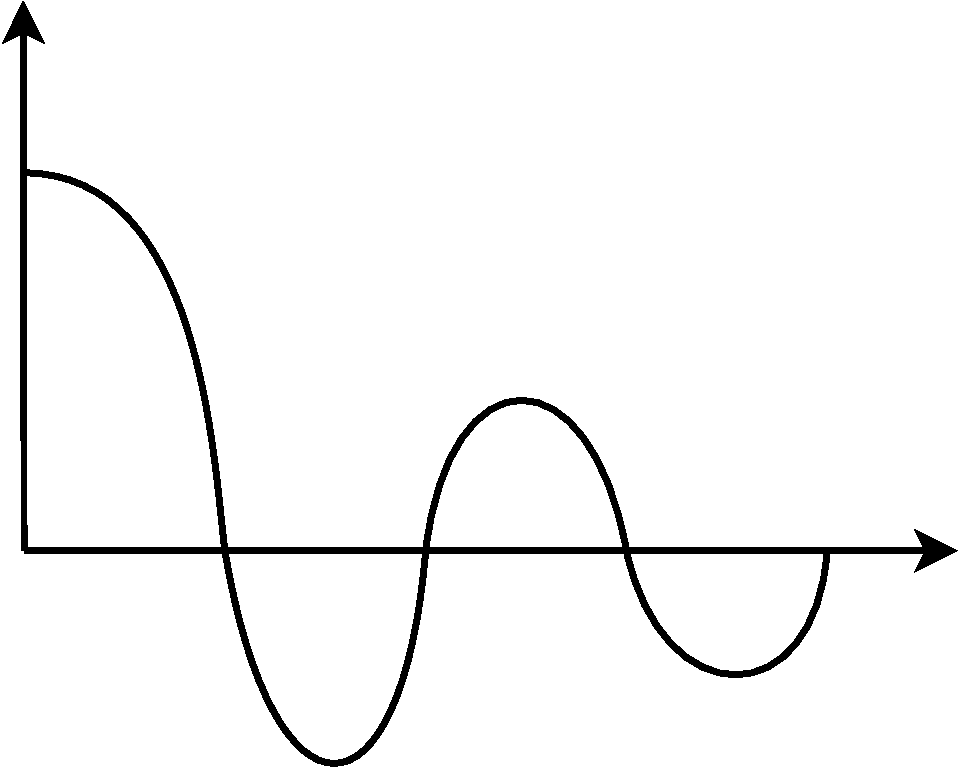
\includegraphics[width=0.6\textwidth]{images/convergentie.png}
    \caption{Grafische voorstelling van de convergentie na een reeks deployment runs.}
    \end{center}
\end{figure}

%CMS laat vaak toe om logisch samenhorende basisobjecten te verzamelen en   
Databases en webserver zijn abstracties die bestaan uit een verzameling basisobjecten zoals bestanden, packages en services.
Tussen deze objecten bestaan er natuurlijk ook afhankelijkheden, bijvoorbeel tussen een bestand en de map waarin het staat:
als de CMS eerst probeert het bestand te cree\"eren en dan pas de map zal de deployment run slechts gedeeltelijk slagen want een bestand kan niet bestaan zonder zijn parent folder.
\begin{figure}
    \label{fig:file_dir_dep}
    \begin{center}
    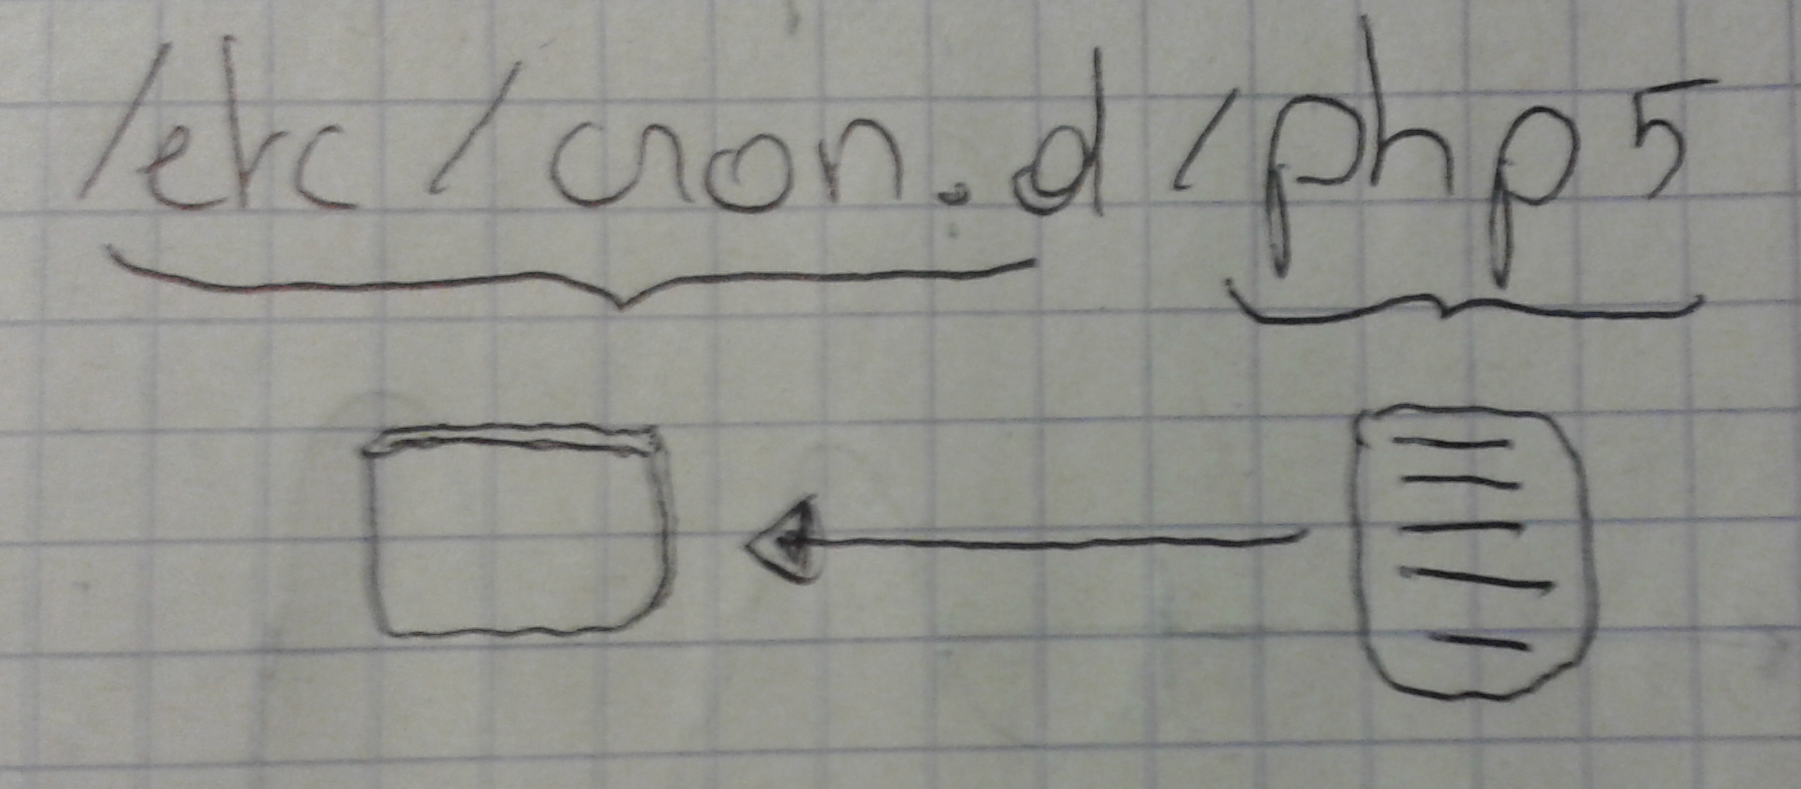
\includegraphics[width=0.6\textwidth]{images/file_dir_dep.png}
    \caption{Grafische voorstelling van de afhankelijkheid tussen een bestand en zijn parent folder}
    \end{center}
\end{figure}
\todo{Hier al eventual consistency vermelden/verwijzen?}

We kunnen dus concluderen dat het vermelden van dependencies in het model het uitrolprocess significant kan verbeteren: als alle afhankelijkheden vermeld zijn is er maar 1 deployment run nodig.
\todo{snelheid nog niet vermeld. Meerdere deployments onnodig maken.}
\todo{Belang: correct gebeuren is van groot belang}

%%%%%%%%%%%%%%%%%%%%%%%%%%%%%%%%%%%%%%%%%%%%%%%%%%%%%
%          Dependencies met huidige tools           %
%%%%%%%%%%%%%%%%%%%%%%%%%%%%%%%%%%%%%%%%%%%%%%%%%%%%%
De huidige CMS laten toe om op het niveau van bestanden, packages en services afhankelijkheden te specifi\"eren.
Bij het uitrollen van een model wordt dan een volgorde opgelegd waarmee de verschillende objecten verwerkt worden.

De tools die momenteel beschikbaar zijn compileren tijdens de deployment voor elke machine hun deel van het model.
Elke machine krijgt dus informatie over wat hijzelf doet maar kan geen rekening houden met wat er op andere machines gebeurt.
Afhankelijkheden binnen \'e\'en machine verwerken is dus geen probleem maar afhankelijkheden tussen verschillende machines zijn niet mogelijk. \todo{Vermelden van workarounds}
De tools die momenteel beschikbaar zijn kunnen dus het hierboven vermelde probleem van een webserver en een database niet oplossen.
%%%%%%%%%%%%%%%%%%%%%%%%%%%%%%%%%%%%%%%%%%%%%%%%%%%%%
%          Dependencies met IMP                     %
%%%%%%%%%%%%%%%%%%%%%%%%%%%%%%%%%%%%%%%%%%%%%%%%%%%%%
IMP (Infrastructure Management Platform) is een nieuwe tool die momenteel nog in ontwikkeling is.
Een andere aanpak tijdens het deployen van een model laat toe afhankelijkheden tussen hoog-niveau objecten te specifi\"eren:
in tegenstelling tot de vorige tools krijgt elke machine het volledige model ter beschikking en niet alleen zijn eigen deel.
Dit laat de machines toe om rekening te houden met afhankelijkheden tussen eigen objecten en die op een andere machine.

%%%%%%%%%%%%%%%%%%%%%%%%%%%%%%%%%%%%%%%%%%%%%%%%%%%%%
%          Probleem/doelstelling                    %
%%%%%%%%%%%%%%%%%%%%%%%%%%%%%%%%%%%%%%%%%%%%%%%%%%%%%
De doelstelling van deze thesis is een effici\"ente manier vinden om een configuratiemodel uit te rollen.
Effici\"ent slaat hier vooral op het vermijden van extra deployment runs door rekening te houden met al dan niet impliciete afhankelijkheden.

%%%%%%%%%%%%%%%%%%%%%%%%%%%%%%%%%%%%%%%%%%%%%%%%%%%%%
%          Kort: hoe oplossing + resultaten         %
%%%%%%%%%%%%%%%%%%%%%%%%%%%%%%%%%%%%%%%%%%%%%%%%%%%%%
